\section{Neural Path Features and Optimisation}
\begin{comment}The ability of DNNs to fit data has been demonstrated in the past. \cite{ben} showed that DNNs can fit even random labels, and random pixels of standard datasets such as MNIST. However, we note that, for standard DNNs with ReLU gates, with no bias parameters, a dataset with $n=2$ points namely $(x,1)$ and $(2x,-1)$ for some $x\in \R^{d_{in}}$ cannot be memorised. The reason is that the gating values are the same for both $x$ and $2x$ (for that matter any positive scaling of $x$), and hence $\phi_{2x,\G_t }= 2\phi_{x,\G_t }$, and thus it not possible to fit arbitrary values for $\hat{y}_t(x)$ and $\hat{y}_t(2x)$.\\
\textbf{How to obtain NPF?}
\end{comment}
In this section, we assume that the gates are held fixed during training (i.e., $\G_t=\G_0,\,\forall\, t\geq 0$, or $\Tg_0=\Tg_0,\,\forall\,t\geq 0$). Thus NPFs are fixed at time $t=0$ and the output is expressed as $\hat{y}_t=\Phi^\top_0 v_t$.  The GD procedure on $\Theta\inrdnet$ learns the values of the path $v_t$. In this scenario, since the feature gradien, $\psi^{\phi}_{x_s,t}=0$, let us look at the value gradient matrix $\Psi^v_t=(\nabla_{\Theta}v_{\Theta_t})^\top \Phi_{\Tg_t}$, where $\nabla_{\Theta}v_{\Theta_t}\in \R^{P\times d_{net}}$ is the collection of the derivatives $\partial_{\theta}v_t(p),\,\forall\,p\in[P],\theta\in\Theta$. The expression for the NTK is given by:
\begin{align}
K_t={\Psi^v}^\top_t\Psi^v_t= \Phi^\top_0(\nabla_{\Theta}v_{\Theta_t})(\nabla_{\Theta}v_{\Theta_t})^\top \Phi_0
\end{align}
\begin{comment}
Now the question of how obtain NPF needs to be addressed. Here, we consider the following two interesting cases:\\
i) \emph{Fixed Random Gating:} For each input example in the dataset, we sample gating values from $Ber(\mu)$ taking values in $\{0,1\}$, and collect it in $\G_0$. This way of generating gates (and hence NPK) is useful for a pure memorisation only task. The reason is that for a new unseen input, there is no natural way of generating the gating values (i.e., NPF) in a manner that will ensure good generalisation.\\
ii) \emph{Parameterised Gating:} A randomly initialised DNN with ReLU activations is a natural choice to provide gating $\G_0$. Since we want the gates to be fixed, the parameters of the gating network is frozen, i.e., $\Tg_0=\Tg_t,\forall\,t\geq 0$, and we can train $\Theta_t$.\\
\end{comment}
We now assume that the gates and the weights are statistically decoupled, and the weights are randomly distributed.
\begin{assumption}\label{assmp:main}
(i) $\Theta_0\inrdnet$  is statistically independent of $\G_0$, (ii) The weights $\Theta_0$ are sampled i.i.d from a distribution such that for any $\theta_0\in\{\Theta_0\cup \Tg_0\}$,  we have $\E{\theta_0}=0$, and  $\E{\theta^2_0}=\sigma^2$, and $\E{\theta^4_0}={\sigma'}^2$.
\end{assumption}
\begin{lemma}\label{lm:disentangle}[Disentanglement] Let $\nabla_{\Theta} v_t\in \R^{P\times d_{net}}$ be matrix whose entries are given by $\nabla_{\Theta} v_t (p,\theta)=\partial_{\theta}v_t(p),\forall p\in [P], \theta\in\Theta$, and let $I_P$ be the $P\times P$ identity matrix. Then, 
under \Cref{assmp:main}-(ii), it follows that $\E{\nabla_{\Theta}v_{\Theta_t})(\nabla_{\Theta}v_{\Theta_t})^\top }= d\sigma^{2(d-1)}I_{P}$.
\end{lemma}
\begin{theorem}\label{th:main} Under \Cref{assmp:main}, we have:\\
(i) $\E{K_0}=\sigma^{2(d-1)}H_0=\sigma^{2(d-1)}(x^\top x)\odot(\lambda_0)$,\\
(ii) In addition, if ${4d}/{w^2}<1$, then $Var\left[K^v_0\right]\leq O\left(d^2_{in}\sigma^{4(d-1)}\max\{d^2w^{2(d-2)+1}, d^3w^{2(d-2)}\}\right)$,\\
\end{theorem}
\begin{comment}
\textbf{Proof of \Cref{th:main}-(i):} Let $\varphi_t=(\varphi_{p,t},p\in[P])\in \R^{d_{net}\times P}$ matrix, then since $K_t=\Psi^\top_t\Psi$, where $\Psi_t=\varphi_t \Phi_t$, we have $\E{K_t}=\E{\Phi^\top_t \varphi^\top_t \varphi_t \Phi_t}$. At initialisation, using the \Cref{assmp:main}-(i), we can pull out $\Phi^\top_t$ and $\Phi_t$ outside of the expectation to have \begin{align}\label{eq:pullout}\E{K_0}=\Phi^\top_0\E{ \varphi^\top_t \varphi_t }\Phi_0,\end{align} and from \Cref{lm:disentangle}, it follows that $\E{ \varphi^\top_t \varphi_t }=d\sigma^{2(d-1)}I$, and hence $\E{K_0}=d\sigma^{2(d-1)}\Phi^\top_0\Phi_0=d\sigma^{2(d-1)}H_0$.\\
\end{comment}
$1.$ \textbf{Active Sub-Network and Gradient Flow:}  Each input example has its own associated set of active sub-network, and while training a particular example, the gradient flows through the weights of the corresponding active sub-network. Now, the active sub-networks corresponding to different examples have some overlap, and hence there is bound to be \emph{cross-talk} of the gradients flowing through them. %This overlap is captured by $\lambda_t(s,s')$ which is the measure of overlap of the sub-networks that are active for both the inputs $x,x'\in\R^{d_{in}}$. Under. \Cref{assmp:main}, the inter-path interaction $\varphi^\top_t\varphi_t$ gets disentangled, result in the claim \Cref{th:main}-(i).\\
$2.$ \textbf{Spectrum of $\lambda_0$} directly controls the spectral properties of the NTK matrix $K_0$. In what follows, we reason that increasing the depth causes whitening of $\lambda_0$.\\%However, in the later part of this section, we consider a special case, wherein, we give an explicit characterisation of the spectrum of $\E{K_0}$. Characterising $\lambda_0$ for the general case is left as future work.\\
$3.$ \textbf{Why increasing depth till a point helps in training? } From \Cref{th:main}-(ii) it follows that for $w\ra\infty$, $K_0\ra\E{K_0}$. We now argue that when $\sigma=\sqrt{\frac{2}{w}}$, increasing depth causes whitening of $\lambda_0$, and hence $K_0$ .\hfill\\
$\bullet$ Let us first look at the diagonal terms of $\lambda_0$. It is reasonable to assume that, owing to the symmetric nature of the weights, roughly $\mu=\frac{1}{2}$ fraction of the gates are \emph{on} every layer. Thus $\lambda_0(s,s)\approx (w/2)^{d-1}$. Now, due our choice of $\sigma=\sqrt{\frac{2}{w}}$, the diagonal entries will be close to $1$.\hfill\\
$\bullet$ We now turn our attention towards the non-diagonal entries of $\lambda_0$. Define $\tau(s,s',l)\stackrel{def}=\sum_{i=1}^w G_{x_s,t}(l,i)G_{x_{s'},t}(l,i)$ be the overlap of the active gates in layer $l$ for input examples $s,s'\in[n]$, and  let $\eta\stackrel{def}=\max_s\left(\max_{s',l} \frac{\tau(s,s',l)}{\tau(s,s,l)}\right)$ be the maximum overlap between gates of a layer (maximum taken over over input pairs $s,s'\in[n]$ and layers $l\in [d]$).  Then it follows that $\max_{s,s'\in [n]} \frac{\bar{\lambda}_{cross}(s,s')}{\bar{\lambda}_{self}(s)}\leq \eta^{d-1}$. Thus, the non-diagonal entries decay an exponential rate in comparison to the diagonal entries.\hfill\\
$4.$ \textbf{Why increasing the depth beyond hurts training?} Note that for $\sigma=O\left(\sqrt{\frac{1}{w}}\right)$, for a fixed depth $d$, as width $w$ increases, $K_0\ra\E{K_0}$. However, the variance expression in \Cref{th:main}-$(ii)$ involves $d^2$ and $d^3$ terms, and hence for a fixed width as depth increases, the entries of $K_0$ deviates from $\E{K_0}$, and as a result the spectrum of $K_0$ degrades, thereby hurting training performance.\\
$5.$ \Cref{assmp:main} is not satisfied by ReLU activations, i.e., conditioned on the fact that a ReLU is \emph{on}, the incoming weights cannot all be simultaneously negative. This implies that the $\Phi^\top_t$ and $\Phi_t$ terms cannot be pulled out of the expectation as in \eqref{eq:pullout}.\\
\begin{wrapfigure}{h}{0.27\textwidth}
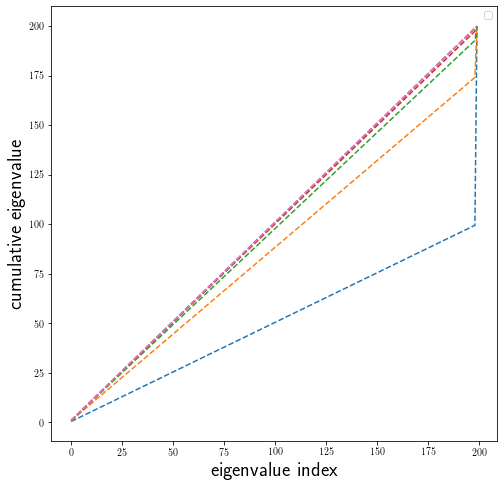
\includegraphics[scale=0.22]{figs/dgn-fra-ecdf-ideal.png}
\caption{Ideal spectrum.}
\label{fig:ideal-spectrum}
\end{wrapfigure}
\begin{comment}
\begin{wrapfigure}{h}{0.27\textwidth}
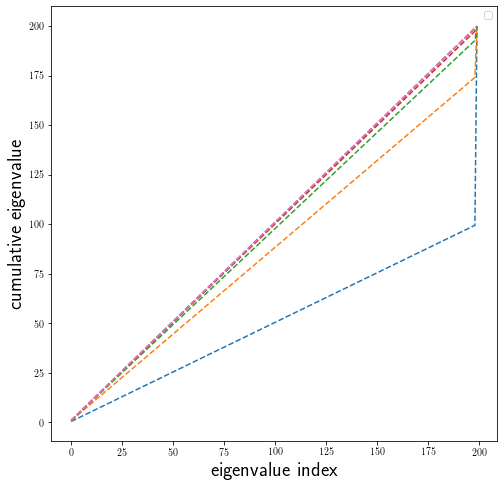
\includegraphics[scale=0.22]{figs/dgn-fra-ecdf-ideal.png}
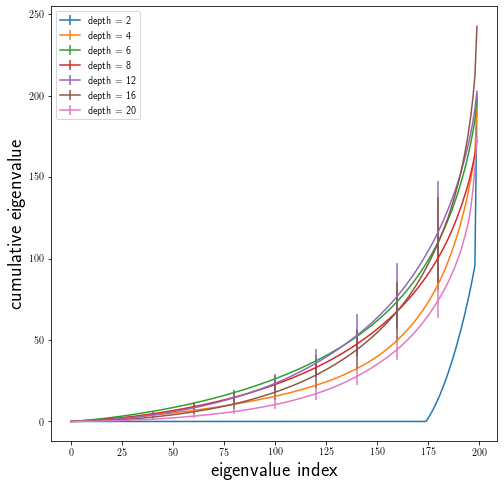
\includegraphics[scale=0.22]{figs/dgn-fra-ecdfbyd-w25.png}
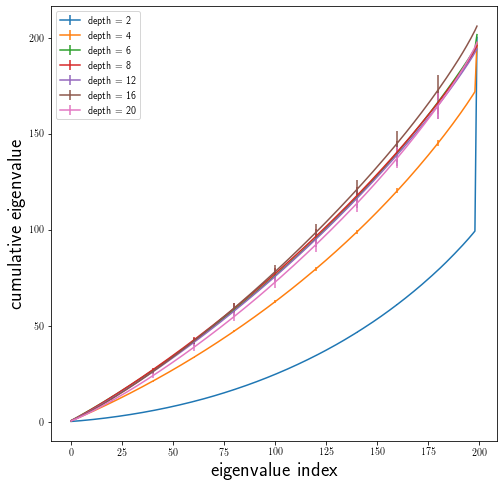
\includegraphics[scale=0.22]{figs/dgn-fra-ecdfbyd-w500.png}
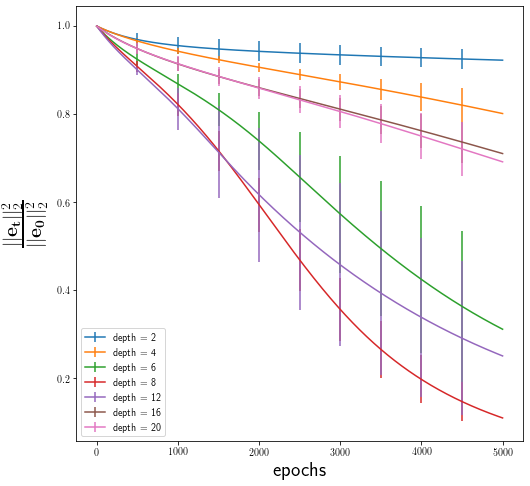
\includegraphics[scale=0.21]{figs/dgn-fra-conv-w25.png}
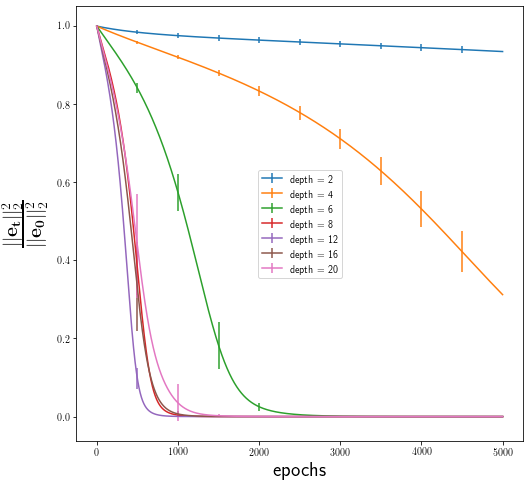
\includegraphics[scale=0.21]{figs/dgn-fra-conv-w500.png}
\caption{Ideal spectrum}
\label{fig:dgn-frg-gram-ecdf}
\end{wrapfigure}
\end{comment}
\textbf{Experiments:} In our experiment, we consider DGNs with the following three different gating schemes namely, i) fixed random (FR): for each input example in the dataset, we sample gating values from $Ber(\mu)$ taking values in $\{0,1\}$, and collect it in $\G_0$. DGN with FR gating is useful only for pure memorisation, ii) fixed explicit (FE): gating parameter $\Tg_t=\Tg_0,\forall\, t\geq 0, \Tg_0\neq \Theta_0$, iii) fixed implicit (FI): gating parameter $\Tg_t=\Tg_0,\forall\, t\geq 0, \Tg_0= \Theta_0$. The FI case does not satisfy \Cref{assmp:main}-(i).
\textbf{Experiment $1$ (DGN-FR):}  In this case, it is easy to check that $\mathbb{E}_{\mu}\left[\lambda_0(s,s)\right]=(\mu w)^{(d-1)},\forall s\in[n]$ and $\mathbb{E}_{\mu}\left[\lambda_0(s,s')\right]=(\mu^2 w)^{(d-1)},\forall s,s'\in[n]$. The
dataset is given by $(x_s,y_s)_{s=1}^n\in \R\times \R$, where $x_s=1,\forall s\in [n]$, and $y_s\sim unif([-1,1])$, $n=200$. The input Gram matrix $x^\top x$ is a $n\times n$ matrix with all entries equal to $1$ and its rank is equal to 1, and hence $H_0=\lambda_0$.\\
\textbf{Spectrum (Theory):} For $\sigma=\sqrt{\frac{1}{\mu w}}$, and by further averaging $\mathbb{E}_{\mu}\left[K_0(s,s)/d\right]=1$, and $\mathbb{E}_{\mu}\left[K_0(s,s')/d\right]=\mu^{(d-1)}$. Now, let $\rho_i\geq 0,i \in [n]$ be the eigenvalues of $\frac{\E{K_0}}{d}$, and let $\rho_{\max}$ and $\rho_{\min}$ be the largest and smallest eigenvalues. \WFclear One can easily show that $\rho_{\max}=1+(n-1)\mu^{d-1}$ and corresponds to the eigenvector with all entries as $1$, and $\rho_{\min}=(1-\mu^{d-1})$ repeats $(n-1)$ times, which corresponds to eigenvectors given by $[0, 0, \ldots, \underbrace{1, -1}_{\text{$i$ and $i+1$}}, 0,0,\ldots, 0]^\top \in \R^n$ for $i=1,\ldots,n-1$.\\
\textbf{Spectrum (numerical):} We look at the cumulative eigenvalue (e.c.d.f) obtained by first sorting the eigenvalues in ascending order then looking at their cumulative sum. The ideal behaviour (top plot of \Cref{fig:dgn-frg-gram-ecdf}) as predicted from theory is that for indices $k\in[n-1]$, the e.c.d.f should increase at a linear rate, i.e., the cumulative sum of the first $k$ indices is equal to $k(1-\mu^{d-1})$, and the difference between the last two indices is $1+(n-1)\mu^{d-1}$. In \Cref{fig:dgn-frg-gram-ecdf}, we plot the actual e.c.d.f for various depths $d=2,4,6,8,12,16,20$ and $w=25,500$ a (second and third from top in \Cref{fig:dgn-frg-gram-ecdf}). \hfill\\
\textbf{Convergence (numerical):} In order to compare how the rate of convergence varies with the depth, we set the step-size $\alpha=\frac{0.1}{\rho_{\max}}$, $w=100$. We use the vanilla SGD-optimiser. Note the$ \frac{1}{\rho_{\max}}$ in the stepsize, ensures that the uniformity of maximum eigenvalue across all the instances, and the convergence should be limited by the smaller eigenvalues. We also look at the convergence rate of the ratio $\frac{\norm{e_t}^2_2}{\norm{e_0}^2_2}$. We notice that for $w=25$, increasing depth till $d=8$ improves the convergence, however increasing beyond $d=8$ worsens the convergence rate. For $w=500$, increasing the depth till $d=12$ improves convergence, and $d=16,20$ are worse than $d=12$.  This matches with the depth phenomena observed in practical DNNs and also matches our theory.\\
\textbf{Experiment $2$:} To characterise the optimisation performance of DGN-FE and DGN-FI networks, we consider the dataset $(x_s,y_s)_{s=1}^{n}\in \R^2\times \R$, where, $x_s\stackrel{iid}\sim unif(\left[-1,1\right]^2)$ and $y_s\stackrel{iid}\sim unif([-1,1])$, $n=100$. The results are shown in \Cref{fig:galu-d}. The rationale behind choosing this data set is that, we want the inputs to be highly correlated by choice.\\
The DGN-FE is similar to DGN-FR case, in that, both e.c.d.f as well as convergence get better with increasing depth. Here too we set the step-size $\alpha=\frac{0.1}{\rho_{\max}}$ (and use vanilla SGD). We also observe that DGN-FE trains faster than DGN-FI and it is also true that the e.c.d.f for the case of  DGN-FE is better than that of DGN-FI. %This can be attributed to the fact that, in DGN-FI network the dot product of two different active paths is not zero and hence the Gram matrix entries fall back to the algebraic expression for $K_t$ in \eqref{eq:ktalg}.
\begin{figure*}[!b]
\resizebox{\textwidth}{!}{
\begin{tabular}{cccc}
%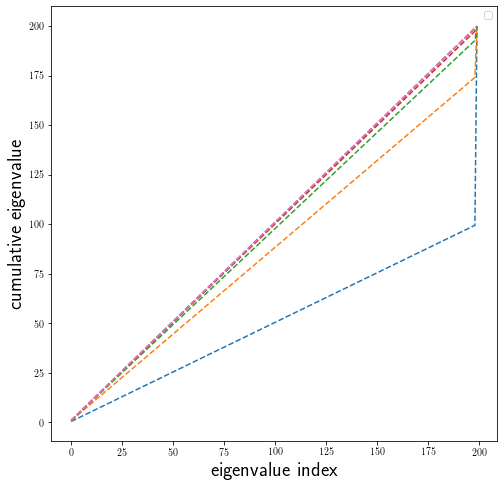
\includegraphics[scale=0.4]{figs/dgn-fra-ecdf-ideal.png}
%&
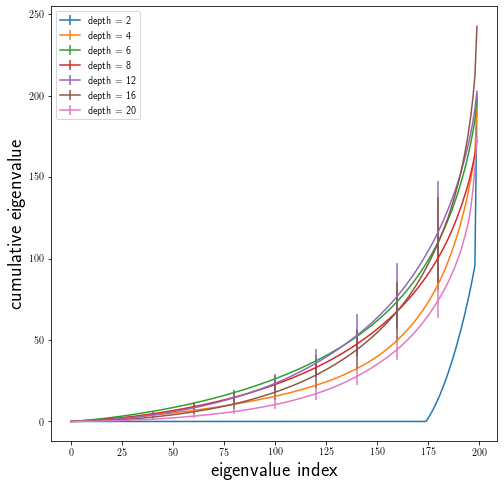
\includegraphics[scale=0.5]{figs/dgn-fra-ecdfbyd-w25.png}
&
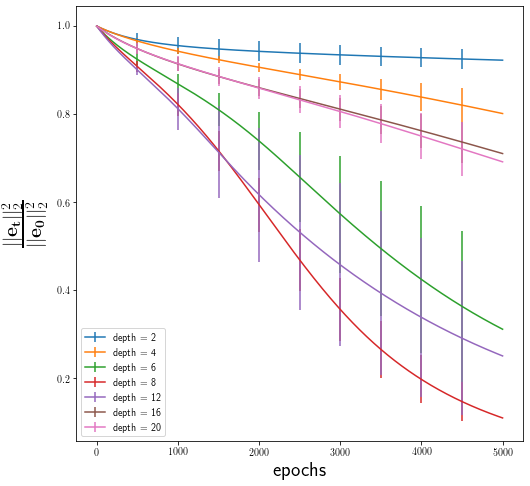
\includegraphics[scale=0.5]{figs/dgn-fra-conv-w25.png}
&
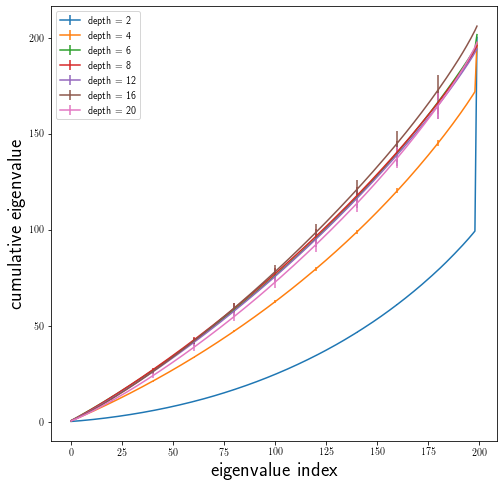
\includegraphics[scale=0.5]{figs/dgn-fra-ecdfbyd-w500.png}
&
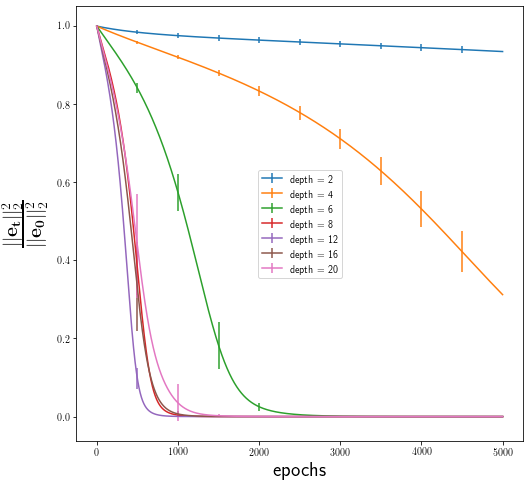
\includegraphics[scale=0.5]{figs/dgn-fra-conv-w500.png}
\end{tabular}
}
\caption{Shows the plots for fixed random gating with $\mu=\frac{1}{2}$ and $\sigma=\sqrt{\frac{2}{w}}$. }
\label{fig:dgn-frg-gram-ecdf}
\end{figure*}

\begin{figure*}[!b]
\resizebox{\textwidth}{!}{
\begin{tabular}{cccc}
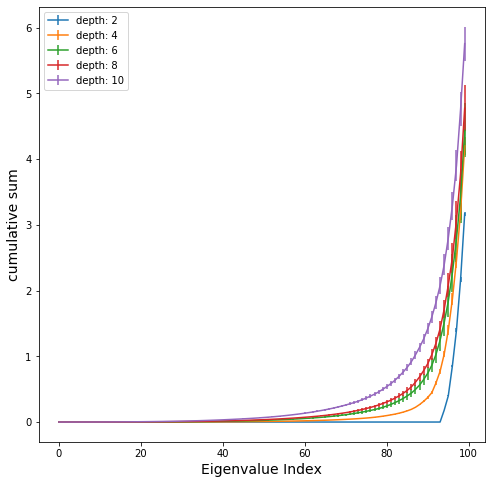
\includegraphics[scale=0.4]{figs/galu-ecdf-d.png}
&
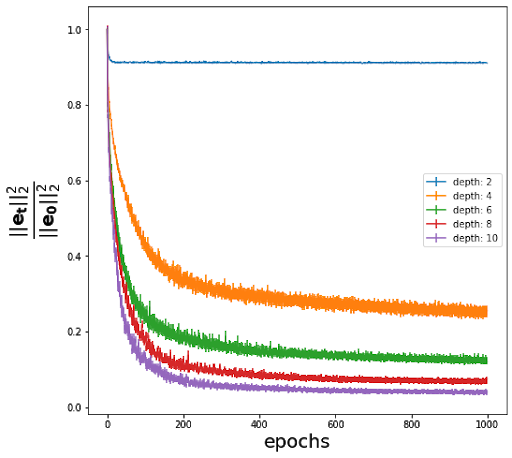
\includegraphics[scale=0.4]{figs/galu-conv-d.png}
&
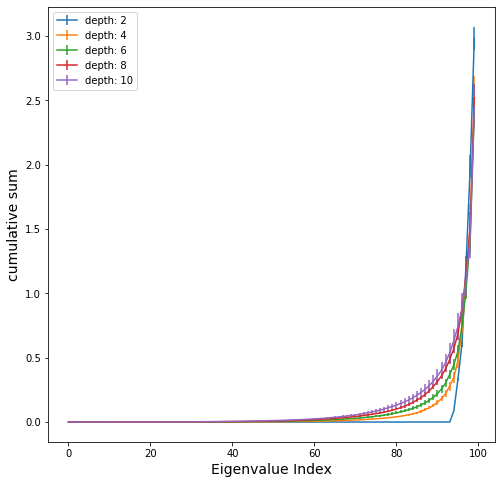
\includegraphics[scale=0.4]{figs/relu-ecdf.png}
&
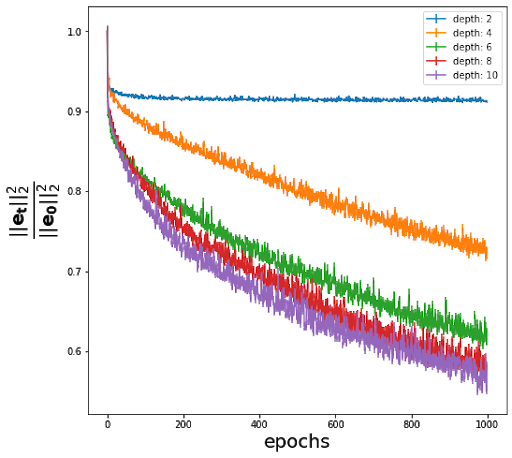
\includegraphics[scale=0.4]{figs/relu-conv.png}
\end{tabular}
}
\caption{The left two plots shows the e.c.d.f and convergence rates for various depth in GaLU networks $w=100$. The third and fourth plot from the left show the e.c.d.f and convergence rates for various depth in ReLU networks $w=100$. The plots are averaged over $5$ runs. }
\label{fig:galu-d}
\end{figure*}
